% Unusual images: what is given as the image of a block.
%  I1. a tcolorbox, breakable or not (it does not break beside the text);
%  I2. a tikzpicture; I3. plain text; I4. nothing;
%  I5. a minipage with a list, a numbered equation and a caption: the
%      numbers are 1, although the image is typeset twice;
%  I6. an image as wide as the line: set above the text, with a warning;
%  I7. an image taller than the page: a warning, and no empty page.
% run.zsh checks that there is no error.
\documentclass{article}
\usepackage{iftex}
\ifPDFTeX
  \usepackage[T1]{fontenc}\usepackage{lmodern}
\fi
\usepackage{graphicx,kantlipsum,tikz,caption}
\usepackage[breakable]{tcolorbox}
\usepackage{wrapblock}
\newcommand\case[2]{\clearpage\section{#1}\begin{wrapblock}{#2}\kant[1]\end{wrapblock}After the block.}
\begin{document}
\case{I1 breakable tcolorbox}{\begin{tcolorbox}[breakable,width=5cm]\kant[2][1-3]\end{tcolorbox}}
\case{I1 tcolorbox}{\begin{tcolorbox}[width=5cm]\kant[2][1-3]\end{tcolorbox}}
\case{I2 tikzpicture}{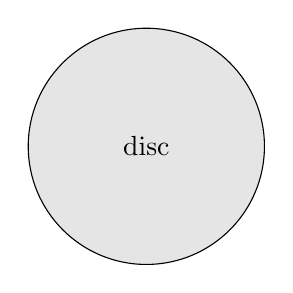
\begin{tikzpicture}\draw[fill=gray!20] (0,0) circle (1.5); \node {disc};\end{tikzpicture}}
\case{I3 text}{Some text given as the image}
\case{I4 nothing}{}
\case{I5 minipage}{\begin{minipage}{5cm}\begin{itemize}\item a first item\item a second one\end{itemize}\begin{equation} a = b \end{equation}\centering\rule{3cm}{1cm}\captionof{figure}{A caption}\end{minipage}}
\case{I6 wide}{\rule{0.95\linewidth}{2cm}}
\case{I7 tall}{\rule{3cm}{1.3\textheight}}
\end{document}
